\documentclass[
  captions=tableheading,
  bibliography=totoc, 
  titepage=firstiscover,
]{scrartcl}

\usepackage{blindtext} %neuer input

\usepackage{longtable} % Tabellen über mehrere Seiten

\usepackage[utf8]{inputenc} %neuer input

\usepackage{scrhack}

\usepackage[aux]{rerunfilecheck} %Warnung falls nochmal kompiliert werden muss

\usepackage{fontspec} %Fonteinstellungen

\recalctypearea{}

\usepackage[main=ngerman]{babel} %deutsche Spracheinstellung

\usepackage{ragged2e} %neuer input

\usepackage{amsmath, nccmath}

\usepackage{amssymb} %viele mathe Symbole

\usepackage{mathtools} %Erweiterungen für amsmath


\DeclarePairedDelimiter{\abs}{\lvert}{\rvert}
\DeclarePairedDelimiter{\norm}{\lVert}{\rVert}

\DeclarePairedDelimiter{\bra}{\langle}{\rvert}
\DeclarePairedDelimiter{\ket}{\lvert}{\rangle}

\DeclarePairedDelimiterX{\braket}[2]{\langle}{\rangle}{
#1 \delimsize| #2
}

\NewDocumentCommand \dif {m}
{
\mathinner{\symup{d} #1}
}


\usepackage[
  math-style=ISO,
  bold-style=ISO,
  sans-style=italic,
  nabla=upright,
  partial=upright,
  warnings-off={
    mathtools-colon,
    mathtools-overbracket,
  },
]{unicode-math}

\setmathfont{Latin Modern Math}
\setmathfont{XITS Math}[range={scr, bfscr}]
\setmathfont{XITS Math}[range={cal, bfcal}, StylisticSet=1]


\usepackage[
  locale=DE,
  separate-uncertainty=true,
  per-mode=reciprocal,
  output-decimal-marker={,},
]{siunitx}

\usepackage[autostyle]{csquotes} %richtige Anführungszeichen

\usepackage{xfrac}

\usepackage{float}

\floatplacement{figure}{htbp}

\floatplacement{table}{htbp}

\usepackage[ %floats innerhalb einer section halten
  section,   %floats innerhalb er section halten
  below,     %unterhalb der Section aber auf der selben Seite ist ok
]{placeins}

\usepackage[
  labelfont=bf,
  font=small,
  width=0.9\textwidth,
]{caption}

\usepackage{subcaption} %subfigure, subtable, subref

\usepackage{graphicx}

\usepackage{grffile}

\usepackage{booktabs}

\usepackage{microtype} %Verbesserungen am Schriftbild

\usepackage[
backend=biber,
]{biblatex}

\addbibresource{../lit.bib}

\usepackage[ %Hyperlinks im Dokument
  german,
  unicode,
  pdfusetitle,
  pdfcreator={},
  pdfproducer={},
]{hyperref}

\usepackage{bookmark}

\usepackage[shortcuts]{extdash}

%\usepackage{warpcol}


\begin{document}
    \title{ATP Übungsblatt 1}
    \author{  
    Tobias Rücker\\
    \texorpdfstring{\href{mailto:tobias.ruecker@tu-dortmund.de}{tobias.ruecker@tu-dortmund.de}
    \and}{,} 
    Paul Störbrock\\
    \texorpdfstring{\href{mailto:paul.stoerbrock@tu-dortmund.de}{paul.stoerbrock@tu-dortmund.de}}{}
    }
\maketitle
\center{\Large Abgabegruppe: \textbf{Mittw. 10-12 Uhr}}
\thispagestyle{empty}

\newpage
\tableofcontents
\thispagestyle{empty}
\newpage

\setcounter{page}{1}


\section{Aufgabe 4}

    \begin{figure}[H]
        \centering
        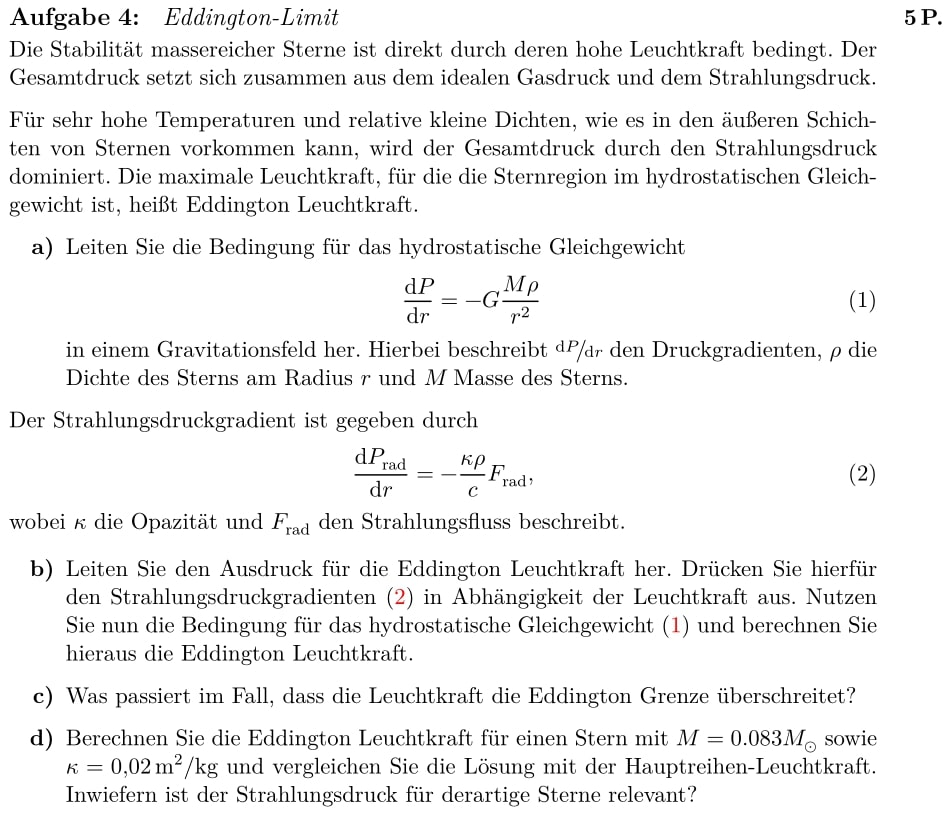
\includegraphics[width=\textwidth]{images/Aufgabe4.jpg}
        \label{fig:1}
    \end{figure}

    \flushleft{Die\;}\justifying Leuchtkraft oder Luminosität eines Sterns ist gegeben durch das Stefan-Boltzman-Gesetzt:
    \begin{align}
        L =  \sigma \cdot A \cdot T^4 \label{eq:1}
    \intertext{flushleft{Wobei\;}\justifying A die betrachtete Oberfläche, T die Oberflächentemperatur und $\sigma = \sfrac{2\pi^5 \kappa^4}{15c^2 h^3}$ die Stefan-Boltzman Konstante darstellt.
    Die Formel des Strahlungsfluss lautet
    }
        f = \frac{P_{Stern}}{A} \label{eq:2}
    \end{align}

\subsection{a)}

    \begin{align*}
        \intertext{\flushleft{Das\;}\justifying hydrostatische Gleichgewicht basiert auf das Gleichgewicht zwischen Strahlung und Druck. Demnach muss eine Variation in Druck oder Strahlung eine entsprechende
        Reaktion der anderen Kraft hervorrufen. Am Equillibrium $F_g = F_p$ muss der Druck der Strahlung gleich der Gewichtskraft sein.
        Die Gewichtskraft, die an der relevanten Schicht herrscht, ist wie folgt definiert:
        }
        F_g &= -G \frac{M_r \mathrm{d}m}{r^2} = -G \frac{M_r \rho}{r^2}\mathrm{d}A \mathrm{d}r
        \intertext{flushleft{Wobei\;}\justifying $G$ die Gravitationskonstante, $M_r$ die Masse der vom Radius $r$ eingeschlossenen Sphäre und $\rho$ die Dichte der Schicht an der Stelle $r$ ist.
        Der Druck ist definiert durch:
        }
        P &= \frac{\text{Kraft(F)}}{\text{Fl\"ache(A)}} \Leftrightarrow F_p = P \cdot A
        \intertext{flushleft{Druck\;}\justifying $p$ und Fläche sind hier jeweils variabel und vom Radius abhängig:
        }
        F_p &= \mathrm{d}P \, \mathrm{d}A
        \intertext{flushleft{Im\;}\justifying perfektem Gleichgewicht müssen sich beide Kräfte aufheben, demnach gilt:
        }
        F_p - F_g &= 0 \Leftrightarrow F_p = F_g\\
        \stackrel{einsetzen}{\Rightarrow} \mathrm{d}P \, \mathrm{d}A &= -G \frac{M_r \rho}{r^2}\mathrm{d}A \mathrm{d}r\\
        \Leftrightarrow \frac{\mathrm{d}P}{\mathrm{d}r} &= -G \frac{M_r \rho}{r^2}
    \end{align*}

\subsection{b)}

    \begin{align*}
        \intertext{flushleft{Für\;}\justifying die Eddington Leuchtkraft wird der Strahlungsfluss \eqref{eq:2} benötigt, welcher in den Strahlungsdruckgradienten für $F_{rad}$ eingesetzt wird. 
        Für den Strahlungsfluss muss die Luminosität am Ort $R$ bekannt sein, welcher sich mit Formel \eqref{eq:1} bestimmen lässt.
        Werden beide Formeln in den Strahlungsdruckgradienten eingesetzt, ergibt sich für $\frac{\mathrm{d}P}{\mathrm{d}r}$:
        }
        \frac{\mathrm{d}P}{\mathrm{d}r} &= -\frac{\kappa \rho}{c} \cdot \frac{L}{A}\\
        \intertext{flushleft{Wird\;}\justifying der Strahlungsdruckgradienten in Abhängigkeit von L nun nach mit der Gewichtskraft gleichgesetzt und nach L umgeformt, ergibt sich:
        }
        -\frac{\kappa \rho}{c} \frac{L}{4\pi r^2} &= -G \frac{M_r \rho}{r^2}\\
        \Leftrightarrow L &= G \frac{4\pi M_r c}{\kappa}
    \end{align*}

\subsection{c)}

    flushleft{Eine\;}\justifying Überschreitung der Eddington Leuchtkraft liegt in der Regel einem zu hohem Strahlungsdruck zugrunde. Ein überwiegender Strahlungsdruck hat in der Regel
    eine Abstrahlung von Masse in Form von Supernovae oder planetaren Nebeln. In beiden Fällen wird mindesten eine Schicht des Stern von der sterneigenen Strahlung abgetragen. 

\subsection{d)}

    \begin{align*}
        \intertext{flushleft{Mit\;}\justifying einer Masse von $0.083 M_{\odot}$ und einer Opazität von \SI{0.02}{\meter\squared\per\kilo\gram} ergibt sich eine Leuchtkraft von:
        } 
        L &= G \frac{4\pi \cdot 0.083 M_{\odot} \cdot c}{\text{\SI{0.02}{\meter\squared\per\kilo\gram}}} = \text{\input{L.tex}}
    \end{align*}

\section{Aufgabe 5}

\begin{figure}[H]
    \centering
    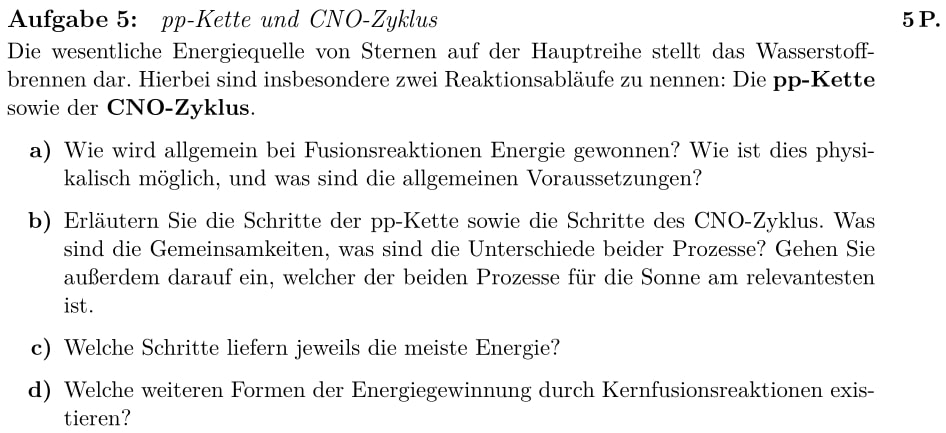
\includegraphics[width=\textwidth]{images/Aufgabe5.jpg}
    \label{fig:2}
\end{figure}

\subsection{a)}

\subsection{b)}

\subsection{c)}

\subsection{d)}


\section{Aufgabe 6}

\begin{figure}[H]
    \centering
    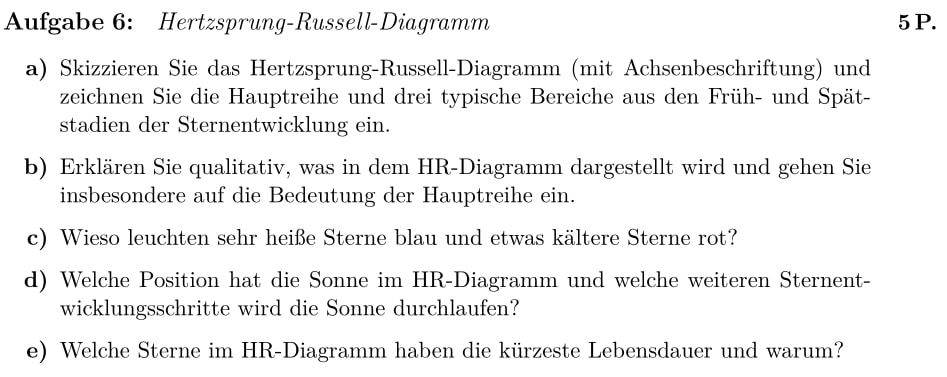
\includegraphics[width=\textwidth]{images/Aufgabe6.jpg}
    \label{fig:3}
\end{figure}

\subsection{a)}

\subsection{b)}

\subsection{c)}

\subsection{d)}

\subsection{e)}






\end{document}